%
%% created with 'latex1html4file' on 2018_02_24@18:41
%
\documentclass[12pt,twocolumn,french]{article}
\usepackage[T1]{fontenc}
\usepackage{float}
\usepackage[utf8]{inputenc}
\usepackage[a4paper]{geometry}
\geometry{verbose,tmargin=15mm,bmargin=15mm,lmargin=15mm,rmargin=15mm}
\usepackage{graphicx}
\usepackage{babel}
\addto\captionsfrench{
\renewcommand{\figurename}{Ph.}
}
\usepackage{tocloft}
\renewcommand{\cftsecleader}{\cftdotfill{\cftdotsep}}
%
\begin{document}
\title{Exemple avec phoges-fik.txt}
\author{Madeleine}
\date{Le samedi 24 février 2018 à 18 heures et 41 minutes}
\maketitle
\tableofcontents \newpage
%
\section{ Tout au Début}
%
  \begin{figure}[H]
    \caption{
       (N=phoges-pic01.jpg)
       (Quand: ??? )
       (Où:  petite place seule )
       (Qui: ??? )
       (Clé(s): ??? )
       (Catégorie(s): ??? )
       (Commentaires: ??? )
    }
    \vspace{4mm}
    \label{phoges-pic01.jpg}
    \noindent \centering{}
    \begin{tabular}{|c|}
      \hline
          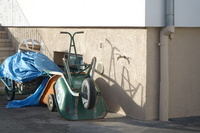
\includegraphics[origin=c,angle=0]{phoges-pic01.jpg}
        \tabularnewline \hline
    \end{tabular}
  \end{figure}

 Il était parti, seul avec son cheval sans provision. 

 Personne, même pas lui n'aurais pu dire où le conduirait sa quête. 

 Ce qui est clair, c'est qu'il y mettait toute son énergie et bientôt le pauvre canasson, harrassé, assoiffé demanda grâce ! 

  \begin{figure}[H]
    \caption{
      [1,1]~: 
       (N=phoges-pic02.jpg)
       (Quand: ??? )
       (Où:  place 2//place 3 )
       (Qui: ??? )
       (Clé(s): boum / place 1 / tic-tac)
       (Catégorie(s): a / b / c)
       (Commentaires: ??? )
      [2,1]~: 
       (N=phoges-pic03.jpg)
       (Quand: ??? )
       (Où:  images nettes//place cinq//place 2//place 3 )
       (Qui: Jeanie)
       (Clé(s): place 1)
       (Catégorie(s): ??? )
       (Commentaires: ??? )
    }
    \vspace{4mm}
    \label{phoges-pic02.jpg}
    \noindent \centering{}
    \begin{tabular}{|c|c|}
      \hline
          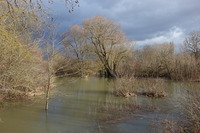
\includegraphics[origin=c,angle=0,width=6cm ]{phoges-pic02.jpg}
        \tabularnewline \hline
          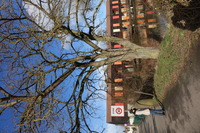
\includegraphics[origin=c,angle=-90,width=6cm ,height=5cm]{phoges-pic03.jpg}
        \tabularnewline \hline
    \end{tabular}
  \end{figure}
%
\subsection{ Mais c'était loin d'être fini}
%

 Toujours personne en vue, et le soleil qui commençait à décliner. 

  \begin{figure}[H]
    \caption{
       (N=phoges-pic04.jpg)
       (Quand:  2018 )
       (Où:  place cinq )
       (Qui: Personne)
       (Clé(s): palabra clave premera]]//[[palabra clave / keyword)
       (Catégorie(s): ??? )
       (Commentaires: 5ème en place)
    }
    \vspace{4mm}
    \label{phoges-pic04.jpg}
    \noindent \centering{}
    \begin{tabular}{|c|}
      \hline
          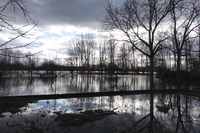
\includegraphics[origin=c,angle=0]{phoges-pic04.jpg}
        \tabularnewline \hline
    \end{tabular}
  \end{figure}
%
\section{ Il fallait aller encore plus loin}
%
  \begin{figure}[H]
    \caption{
       (N=phoges-pic05.jpg)
       (Quand: ??? )
       (Où:  place cinq )
       (Qui: ??? )
       (Clé(s): ??? )
       (Catégorie(s): ??? )
       (Commentaires: aussi la 5ème par individuel)
    }
    \vspace{4mm}
    \label{phoges-pic05.jpg}
    \noindent \centering{}
    \begin{tabular}{|c|}
      \hline
          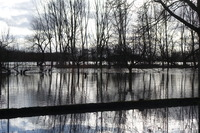
\includegraphics[origin=c,angle=0]{phoges-pic05.jpg}
        \tabularnewline \hline
    \end{tabular}
  \end{figure}
%
\section{ Jamais on n'en voyait la fin}
%

Marcher, toujours marcher sans s'arrêter. Mais un matin, il put distinguer de la poussière ; accélérant sa marche, il se rapprocha d'un groupe d'étranges personnages.

%
\subsection{ Encore un mirage}
%
  \begin{figure}[H]
    \caption{
       (N=phoges-pic06.jpg)
       (Quand: ??? )
       (Où:  place 3 )
       (Qui: ??? )
       (Clé(s): palabra clave cuarta)
       (Catégorie(s): b / c)
       (Commentaires: 5 et 3)
    }
    \vspace{4mm}
    \label{phoges-pic06.jpg}
    \noindent \centering{}
    \begin{tabular}{|c|}
      \hline
          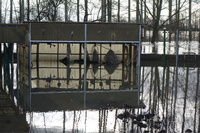
\includegraphics[origin=c,angle=0]{phoges-pic06.jpg}
        \tabularnewline \hline
    \end{tabular}
  \end{figure}
%
\section{ C'est la fin des haricots}
%
  \begin{figure}[H]
    \caption{
       (N=phoges-pic07.jpg)
       (Quand: ??? )
       (Où:  de plus//place 3//place 2 )
       (Qui: ??? )
       (Clé(s): palabra clave segunda / palabra clave premera)
       (Catégorie(s): ??? )
       (Commentaires: ??? )
    }
    \vspace{4mm}
    \label{phoges-pic07.jpg}
    \noindent \centering{}
    \begin{tabular}{|c|}
      \hline
          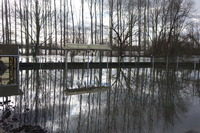
\includegraphics[origin=c,angle=0]{phoges-pic07.jpg}
        \tabularnewline \hline
    \end{tabular}
  \end{figure}
%
\end{document}
%
